%%% The main file. It contains definitions of basic parameters and includes all other parts.

%% Settings for single-side (simplex) printing
% Margins: left 40mm, right 25mm, top and bottom 25mm
% (but beware, LaTeX adds 1in implicitly)
\documentclass[12pt,a4paper]{report}
\setlength\textwidth{145mm}
\setlength\textheight{247mm}
\setlength\oddsidemargin{15mm}
\setlength\evensidemargin{15mm}
\setlength\topmargin{0mm}
\setlength\headsep{0mm}
\setlength\headheight{0mm}
% \openright makes the following text appear on a right-hand page
\let\openright=\clearpage

%% Settings for two-sided (duplex) printing
% \documentclass[12pt,a4paper,twoside,openright]{report}
% \setlength\textwidth{145mm}
% \setlength\textheight{247mm}
% \setlength\oddsidemargin{14.2mm}
% \setlength\evensidemargin{0mm}
% \setlength\topmargin{0mm}
% \setlength\headsep{0mm}
% \setlength\headheight{0mm}
% \let\openright=\cleardoublepage

%% Character encoding: usually latin2, cp1250 or utf8:
\usepackage[utf8]{inputenc}

%% Further useful packages (included in most LaTeX distributions)
\usepackage{amsmath}        % extensions for typesetting of math
\usepackage{amsfonts}       % math fonts
\usepackage{amsthm}         % theorems, definitions, etc.
\usepackage{bbding}         % various symbols (squares, asterisks, scissors, ...)
\usepackage{bm}             % boldface symbols (\bm)
\usepackage{graphicx}       % embedding of pictures
\usepackage{fancyvrb}       % improved verbatim environment
\usepackage{natbib}         % citation style AUTHOR (YEAR), or AUTHOR [NUMBER]
\usepackage[nottoc]{tocbibind} % makes sure that bibliography and the lists
			    % of figures/tables are included in the table
			    % of contents
\usepackage{dcolumn}        % improved alignment of table columns
\usepackage{booktabs}       % improved horizontal lines in tables
\usepackage{paralist}       % improved enumerate and itemize
\usepackage[usenames]{xcolor}  % typesetting in color

%%% Basic information on the thesis

% Thesis title in English (exactly as in the formal assignment)
\def\ThesisTitle{Web data extraction language}

% Author of the thesis
\def\ThesisAuthor{Tomáš Novella}

% Year when the thesis is submitted
\def\YearSubmitted{2016}

% Name of the department or institute, where the work was officially assigned
% (according to the Organizational Structure of MFF UK in English,
% or a full name of a department outside MFF)
\def\Department{Department of Software Engineering}

% Is it a department (katedra), or an institute (ústav)?
\def\DeptType{Department}

% Thesis supervisor: name, surname and titles
\def\Supervisor{RNDr. Irena Holubová, Ph.D}

% Supervisor's department (again according to Organizational structure of MFF)
\def\SupervisorsDepartment{department}

% Study programme and specialization
\def\StudyProgramme{Informatics}
\def\StudyBranch{study branch}

% An optional dedication: you can thank whomever you wish (your supervisor,
% consultant, a person who lent the software, etc.)
\def\Dedication{%
Dedication.
}

% Abstract (recommended length around 80-200 words; this is not a copy of your thesis assignment!)
\def\Abstract{%
Abstract.
}

% 3 to 5 keywords (recommended), each enclosed in curly braces
\def\Keywords{%
{key} {words}
}

%% The hyperref package for clickable links in PDF and also for storing
%% metadata to PDF (including the table of contents).
\usepackage[pdftex,unicode]{hyperref}   % Must follow all other packages
\hypersetup{breaklinks=true}
\hypersetup{pdftitle={\ThesisTitle}}
\hypersetup{pdfauthor={\ThesisAuthor}}
\hypersetup{pdfkeywords=\Keywords}
\hypersetup{urlcolor=blue}

% Definitions of macros (see description inside)
%%% This file contains definitions of various useful macros and environments %%%
%%% Please add more macros here instead of cluttering other files with them. %%%

%%% Minor tweaks of style

% These macros employ a little dirty trick to convince LaTeX to typeset
% chapter headings sanely, without lots of empty space above them.
% Feel free to ignore.
\makeatletter
\def\@makechapterhead#1{
  {\parindent \z@ \raggedright \normalfont
   \Huge\bfseries \thechapter. #1
   \par\nobreak
   \vskip 20\p@
}}
\def\@makeschapterhead#1{
  {\parindent \z@ \raggedright \normalfont
   \Huge\bfseries #1
   \par\nobreak
   \vskip 20\p@
}}
\makeatother

% This macro defines a chapter, which is not numbered, but is included
% in the table of contents.
\def\chapwithtoc#1{
\chapter*{#1}
\addcontentsline{toc}{chapter}{#1}
}

% Draw black "slugs" whenever a line overflows, so that we can spot it easily.
\overfullrule=1mm

%%% Macros for definitions, theorems, claims, examples, ... (requires amsthm package)

\theoremstyle{plain}
\newtheorem{thm}{Theorem}
\newtheorem{lemma}[thm]{Lemma}
\newtheorem{claim}[thm]{Claim}

\theoremstyle{plain}
\newtheorem{defn}{Definition}

\theoremstyle{remark}
\newtheorem*{cor}{Corollary}
\newtheorem*{rem}{Remark}
\newtheorem*{example}{Example}

%%% An environment for proofs

%%% FIXME %%% \newenvironment{proof}{
%%% FIXME %%%   \par\medskip\noindent
%%% FIXME %%%   \textit{Proof}.
%%% FIXME %%% }{
%%% FIXME %%% \newline
%%% FIXME %%% \rightline{$\square$}  % or \SquareCastShadowBottomRight from bbding package
%%% FIXME %%% }

%%% An environment for typesetting of program code and input/output
%%% of programs. (Requires the fancyvrb package -- fancy verbatim.)

\DefineVerbatimEnvironment{code}{Verbatim}{fontsize=\small, frame=single}

%%% The field of all real and natural numbers
\newcommand{\R}{\mathbb{R}}
\newcommand{\N}{\mathbb{N}}

%%% Useful operators for statistics and probability
\DeclareMathOperator{\pr}{\textsf{P}}
\DeclareMathOperator{\E}{\textsf{E}\,}
\DeclareMathOperator{\var}{\textrm{var}}
\DeclareMathOperator{\sd}{\textrm{sd}}

%%% Transposition of a vector/matrix
\newcommand{\T}[1]{#1^\top}

%%% Various math goodies
\newcommand{\goto}{\rightarrow}
\newcommand{\gotop}{\stackrel{P}{\longrightarrow}}
\newcommand{\maon}[1]{o(n^{#1})}
\newcommand{\abs}[1]{\left|{#1}\right|}
\newcommand{\dint}{\int_0^\tau\!\!\int_0^\tau}
\newcommand{\isqr}[1]{\frac{1}{\sqrt{#1}}}

%%% Various table goodies
\newcommand{\pulrad}[1]{\raisebox{1.5ex}[0pt]{#1}}
\newcommand{\mc}[1]{\multicolumn{1}{c}{#1}}


% Title page and various mandatory informational pages
\begin{document}
%%% Title page of the thesis and other mandatory pages

%%% Title page of the thesis

\pagestyle{empty}
\hypersetup{pageanchor=false}
\begin{center}

\large

Charles University in Prague

\medskip

Faculty of Mathematics and Physics

\vfill

{\bf\Large MASTER THESIS}

\vfill

\centerline{\mbox{\includegraphics[width=60mm]{../img/logo.pdf}}}

\vfill
\vspace{5mm}

{\LARGE\ThesisAuthor}

\vspace{15mm}

{\LARGE\bfseries\ThesisTitle}

\vfill

\Department

\vfill

\begin{tabular}{rl}

Supervisor of the master thesis: & \Supervisor \\
\noalign{\vspace{2mm}}
Study programme: & \StudyProgramme \\
\noalign{\vspace{2mm}}
Study branch: & \StudyBranch \\
\end{tabular}

\vfill

% Zde doplňte rok
Prague \YearSubmitted

\end{center}

\newpage

%%% Here should be a bound sheet included -- a signed copy of the "master
%%% thesis assignment". This assignment is NOT a part of the electronic
%%% version of the thesis. DO NOT SCAN.

%%% A page with a solemn declaration to the master thesis

\openright
\hypersetup{pageanchor=true}
\pagestyle{plain}
\pagenumbering{roman}
\vglue 0pt plus 1fill

\noindent
I declare that I carried out this master thesis independently, and only with the cited
sources, literature and other professional sources.

\medskip\noindent
I understand that my work relates to the rights and obligations under the Act No.~121/2000 Sb.,
the Copyright Act, as amended, in particular the fact that the Charles
University in Prague has the right to conclude a license agreement on the use of this
work as a school work pursuant to Section 60 subsection 1 of the Copyright Act.

\vspace{10mm}

\hbox{\hbox to 0.5\hsize{%
In ........ date ............	% FIXME!
\hss}\hbox to 0.5\hsize{%
signature of the author
\hss}}

\vspace{20mm}
\newpage

%%% Mandatory information page of the thesis

\openright

\vbox to 0.5\vsize{
\setlength\parindent{0mm}
\setlength\parskip{5mm}

Title:
\ThesisTitle

Author:
\ThesisAuthor

\DeptType:
\Department

Supervisor:
\Supervisor, \SupervisorsDepartment

Abstract:
\Abstract

Keywords:
\Keywords

\vss}

\newpage

%%% Dedication

\openright

\noindent
\Dedication

\newpage

\openright
\pagestyle{plain}
\pagenumbering{arabic}
\setcounter{page}{1}


%%% A page with automatically generated table of contents of the master thesis

\tableofcontents

%%% Each chapter is kept in a separate file
\chapter{Introduction}

Since the dawn of the Internet, the amount of information available has been multiplying every year. Email, Social networks, Mashups, Discussions they all contribute to rapid growth of information.

With the increasing mass of data and growing complexity of its presentation it has become harder than ever to find collections of relevant information.

In the early days, people managed to extract information from the web pages manually,
 or by using simple ad-hoc scripts in general purpose languages.
As the webpages got more complex and deep web got deeper, 
 an increasing need arised, for a system that could scrape data effectively.
These systems, precisely Web Data Extration Systems, have been developed
 using a number of different approaches, which resulted 
in a variety of strengths and weaknesses. 
None of them seems to be accepted by the general public, and so, there cannot even be a community that would 
take care of further \"common\" development of such solution.


In this thesis we will research the pros and cons of the available solutions and will architect a system that will suit a need of a more general public.
That system will have to be sufficiently lightweight, yet effective and would provide a good alernative to the expensive commercial solutions. Our main focus will be laid upon extensionability and quick deployability, in which we believe, we could get the edge against the commercial counterparts. 
Alongside, we will try to point in some directions for the potential further development of the system.

\section{Structure of the Thesis}
This thesis is structured as follows:
Chapter 1 defines the goal of the thesis and defines its structure.
Chapter 2 introduces the taxonomy of the topic and demonstrates the challenges and the use cases and gives rise to
Chapter 3 where we describe the related systems
Chapter 4 that describes our, our contribution, the Serrano language, whilst
Chapter 5 discusses the particular strong and weak points of it and compares it to the rivals whereas
Chapter 6 discusses real-world applications and clients that have used the project 

Q: there should I mention the clients? (avast, adblock, magneto,...) in the last chapter?


Need for extracting information derives from the fact that once extracted, the data can be handled in a way similar to instances of a traditional database.

1.1 Challenges of Web Data Extraction
Q: not sure wher to put it
- human effort - provide a high degree of automation
- check for correctness (data consistency)
- ability to process large volumes of data
- ....
- maintainance - constant change of the web
\chapter{Related work}

An~example citation: \cite{Andel07}

These days, web data extraction is getting more and more important.
\section{Title of the first subchapter of the first chapter}

\section{Title of the second subchapter of the first chapter}

\chapter{Related Work}
In this section we will examine some popular data extraction tools and describe their usage and their benefits along with their drawback. We will present a very popular browser extension named Selenium (\url{http://www.seleniumhq.org/}) to illustrate the state-of-the-art software for browser automaton, then we will inspect 3 different scrapers. First of them, iOpus (\url{http://imacros.net/}), is the most popular browser extension, used for scraping, having over 10 milion downloads, then we will look at Deixto\cite{kokkoras2013deixto}, which is a very popular free software. Then we will describe languages based on extending the XPath language, namely OXPath ans SXPath  and last we will inspect the most popular commercial solution, Lixto\cite{baumgartner2001visual}, which is a GUI around the Elog language.

Because GUI is just a mere wrapper around the language and~it reflects the~strengths and~weaknesses of~the~languages, we will pay most attention to the language.


\section{Selenium}
Selenium (\url{http://www.seleniumhq.org/}) is self-described with a statement \textit{Selenium automates browsers. That's it!} which is an accurate description. Although this tool is not a Web Data Extraction system per se, it shares almost all attributes with them. Moreover, Selenium offers two services, Selenium IDE, which is a browser extension and Selenium WebDriver, which is a collection of bindings to programming languages, so that the user will be able to work with the data after processing.
Nevertheless, the main selling point of the product is testing and automation, i.e. writing automated tests for a web service.

Users can either write custom macros that consist of a list of commands to be executed, or simply press the "Start recording" button and manually perform the actions in the browser. The extension will record the action and generate a wrapper.

Apart from basic commands for navigation, such as filling out the forms, clicking on the buttons and following the links, it is also equipped with testing related functionality, like asserts for a concrete value in a given selector.

This tool provides front-end web testers with unparalleled services to the point that it has become a de facto standard in the web testing stack.

Although the language is fully-equipped for navigation and automation, it lacks in other areas, e.g. it does not provide a mean to transform the extracted data, or to edit the DOM - this functionality is further delegated.

The web-driver wrapper around the language is available in multiple languages, however, it  still does not provide any data transformation capabilities.

\subsection{Example}
We examined this tool by a real-world example, where we logged into Facebook and selected the second most recent conversation.
Source of the macro is in figure~\ref{fig:seleniumCommands}
\begin{figure}
    \centering
    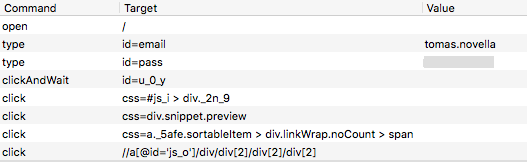
\includegraphics[width=\textwidth]{../img/seleniumCommands}
    \caption{A series of commands that leads to logging into \url{https://www.facebook.com} and choosing the second most recent conversation}
    \label{fig:seleniumCommands}
\end{figure}

\section{iMacros}
This tool, formerly known as iOpus, strongly resembles the Selenium IDE and is in fact targeting a very similar audience. It even provides a website that lists the distinctions between iMacros and Selenium (\url{http://wiki.imacros.net/Selenium}). The use cases differ from Selenium and are as follows:
\begin{enumerate}
    \item Browser Automation
    \item Web Testing
    \item Data Extraction
\end{enumerate}

\subsection{Browser Automation and Web Testing}
In these areas is the tool very similar to Selenium. Form filling and link navigation are standard and 
The command set is very similar, only has different names.
Moreover, it offers a possibility to extract data into variables and to navigate through more complex dynamic pages, supporting sliders (\url{http://maps.google.com}) and drag-and-drop functionality.
Identification of the elements on the page is either by XPath, CSS selectors, or by the element's type, positions and attributes. On top of this, is offers functionality to detect and intercept built-in browser dialogs, such as the download dialog and native Javascript dialogs. A very nice advanced functionality is the image recognition functionality. It relies on the rendering of the image and using advanced neural networks it can identify the element, even if it has moved, or has changed color.

\subsection{Data Extraction}
This is the main differentiator; in this domain, we can select a variable to which the data will be extracted. Plain-text and CSV output formats are supported.
One of the most significant drawbacks is the lack of any structure in the extracted data, it is a simple flat list of data.

\subsection{Example}
Again, we tried to log into Facebook and select the second conversation. Automatic recording broke down, but after some manual effort we made a macro in Figure \ref{fig:iMacrosCommands}.
\begin{figure}
    \centering
    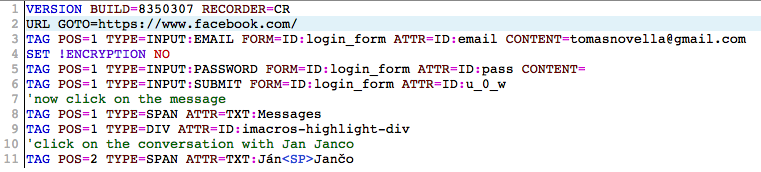
\includegraphics[width=\textwidth]{../img/iMacrosCommands}
    \caption{A series of commands that leads to logging into \url{https://www.facebook.com} and choosing a conversation with Jan Janco.}
    \label{fig:iMacrosCommands}
\end{figure}


\section{XPath-based languages}
In this section we
\subsection{OXPath}
\subsection{SXPath}

\section{Deixto}

\section{Lixto}


\chapter*{Conclusion}
\addcontentsline{toc}{chapter}{Conclusion}

%%% Ukázka použití některých konstrukcí LaTeXu

\subsection{Ukázka \LaTeX{}u}
\label{ssec:ukazka}

This short subsection serves as an~example of basic \LaTeX{} constructs,
which can be useful for writing a~thesis.

Let us start with lists:

\begin{itemize}
\item The logo of Matfyz is displayed in figure~\ref{fig:mff}.
\item This is subsection~\ref{ssec:ukazka}.
\item Citing literature~\cite{lamport94}.
\end{itemize}

Different kinds of dashes:
red-black (short),
pages 16--22 (middle),
$45-44$ (minus),
and this is --- as you could have expected --- a~sentence-level dash,
which is the longest.
(Note that we have follwed \verb|a| by a~tilde instead of a~space
to avoid line breaks at that place.)

\newtheorem{theorem}{Theorem}
\newtheorem*{define}{Definition}	% Definice nečíslujeme, proto "*"

\begin{define}
A~{\sl Tree} is a connected graph with no cycles.
\end{define}

\begin{theorem}
This theorem is false.
\end{theorem}

\begin{proof}
False theorems do not have proofs.
\end{proof}

\begin{figure}
	\centering
	\includegraphics[width=30mm]{../img/logo.pdf}
	\caption{Logo of MFF UK}
	\label{fig:mff}
\end{figure}


%%% Bibliography
\include{Bibliography}

%%% Figures used in the thesis (consider if this is needed)
\listoffigures

%%% Tables used in the thesis (consider if this is needed)
%%% In mathematical theses, it could be better to move the list of tables to the beginning of the thesis.
\listoftables

%%% Abbreviations used in the thesis, if any, including their explanation
%%% In mathematical theses, it could be better to move the list of abbreviations to the beginning of the thesis.
\chapwithtoc{List of Abbreviations}

%%% Attachments to the master thesis, if any. Each attachment must be
%%% referred to at least once from the text of the thesis. Attachments
%%% are numbered.
%%%
%%% The printed version should preferably contain attachments, which can be
%%% read (additional tables and charts, supplementary text, examples of
%%% program output, etc.). The electronic version is more suited for attachments
%%% which will likely be used in an electronic form rather than read (program
%%% source code, data files, interactive charts, etc.). Electronic attachments
%%% should be uploaded to SIS and optionally also included in the thesis on a~CD/DVD.
\chapwithtoc{Attachments}

\openright
\end{document}
